\documentclass[14pt]{extarticle}
\usepackage[utf8]{inputenc}
\usepackage[T1]{fontenc}
\usepackage[spanish,es-lcroman]{babel}
\usepackage{amsmath}
\usepackage{amsthm}
\usepackage{physics}
\usepackage{tikz}
\usepackage{float}
\usepackage[autostyle,spanish=mexican]{csquotes}
\usepackage[per-mode=symbol]{siunitx}
\usepackage{gensymb}
\usepackage{multicol}
\usepackage{enumitem}
\usepackage[left=2.00cm, right=2.00cm, top=2.00cm, 
     bottom=2.00cm]{geometry}
\usepackage{Estilos/ColoresLatex}

\newcommand{\textocolor}[2]{\textbf{\textcolor{#1}{#2}}}

%\renewcommand{\questionlabel}{\thequestion)}
\decimalpoint
\sisetup{bracket-numbers = false}

\title{\vspace*{-2cm} Ejercicios Opcionales - Física 1\vspace{-5ex}}
\date{\today}

\begin{document}
\maketitle

\section{Ejercicios a cuenta}

Con la finalidad de apoyar en la recuperación del promedio para los siguientes exámenes parciales, se dejarán una serie de \textocolor{red}{ejercicios adicionales} para Evaluación Continua.


Estos ejercicios serán de carácter \textocolor{cobalt}{opcional}, es decir, la alumna o alumno que desee resolverlos y enviarlos, les sumará $5$ puntos adicionales a la Evaluación Continua.

La entrega se hará vía Teams en asignación, teniendo como plazo el día domingo 9 de julio a las 8 pm.

Cada ejercicio vale $1$ punto, siempre y cuando esté correcto. Se otorgará una parte proporcional en caso de tener desarrollo detallado pero el resultado no sea el esperado.

Anota en la hoja tu nombre completo, así como una identificación de cada ejercicio.

\begin{enumerate}
\item Realizar la conversión de \SI{7}{\square\meter} a pie$^{2}$.
\item Una lancha de motor efectúa los siguientes desplazamientos: \SI{300}{\meter} al oeste, \SI{200}{\meter} al norte, \SI{350}{\meter} al noreste y \SI{150}{\meter} al sur.
\begin{enumerate}[label=\alph*)]
\item ¿Qué distancia total recorre?
\item Determina gráficamente, ¿cuál es su desplazamiento resultante, en qué dirección actúa, y cuál es el valor de su ángulo medido respecto al oeste? Tendrás que hacer uso de tu juego de geometría y de preferencia en un papel cuadriculado.
\end{enumerate}
\item Con una cuerda, un niño jala un carro con una fuerza de \SI{80}{\newton}, la cual forma un ángulo de $\ang{40}$ con el eje horizontal como se puede observar en la figura:
\begin{figure}[H]
     \centering
     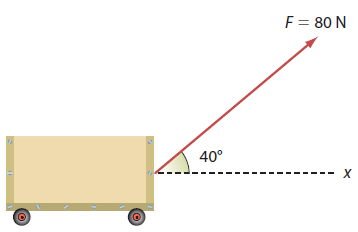
\includegraphics[scale=1]{Imagenes/Ejercicio_Opcional_01.png}
\end{figure}
Calcula:
\begin{enumerate}[label=\alph*)]
\item La magnitud de la fuerza que jala el carro horizontalmente.
\item La magnitud de la fuerza que tiende a levantar al carro.
\end{enumerate}
\item Realiza la siguiente operación en notación científica, debiendo de hacer el manejo en todo momento con la notación:
\begin{align*}
\dfrac{\num{6.1d18}}{\num{7.5d7}} + \num{7d9} - \left[ \left( \num{4.51d-5} \right) \left( \num{2.3d-2} \right)\right]
\end{align*}
\item Se desea conocer cuántos litros de agua le caben a una alberca olímpica de \SI{50}{\meter} de largo,
\SI{25}{\meter} de ancho y \SI{2.7}{\meter} de profundidad.
\end{enumerate}

\end{document}